\section{Fullskala simulering}
\subsection{Oppsett}
Med simuleringsblokkene klare og eit simuleringsvindauge til å vise resultat, var vi no klare for simulering av reinseanlegget.
Vi implementerte ventil-simuleringsblokka på alle ventilane i programmet og oppretta eit
nytt \gls{CFC} vindauge som kopla tanksimuleringa av mottakstanken og reaktorane saman med resten av
programmet.

Simuleringa er sett opp slik at tilstrøyminga til anlegget kan justerast via ein glidebrytar.
Dersom ein av reaktorane er i innpumpingssekvens, simulerer vi flytting av avlaupsvatn basert på pumpekurver og løftehøgde.

Reaktortilstand er presentert med ein tekstvariabel, og
dei aktuelle tidsparameterane, som t.d. tid for reaksjonssekvens,
er redusert for å akselerere simuleringa.

Vi har oppretta eit varslingsystem for alle moglege varslingar anlegget kan generere, uavhengig om dei er relevante for sluttprogrammet.
Dette gir oss verdifull innsikt i eventuelle feil som oppstår og korleis programmet verkar.

\thispagestyle{fancy}
\begin{figure}[htbp]
    \centering
    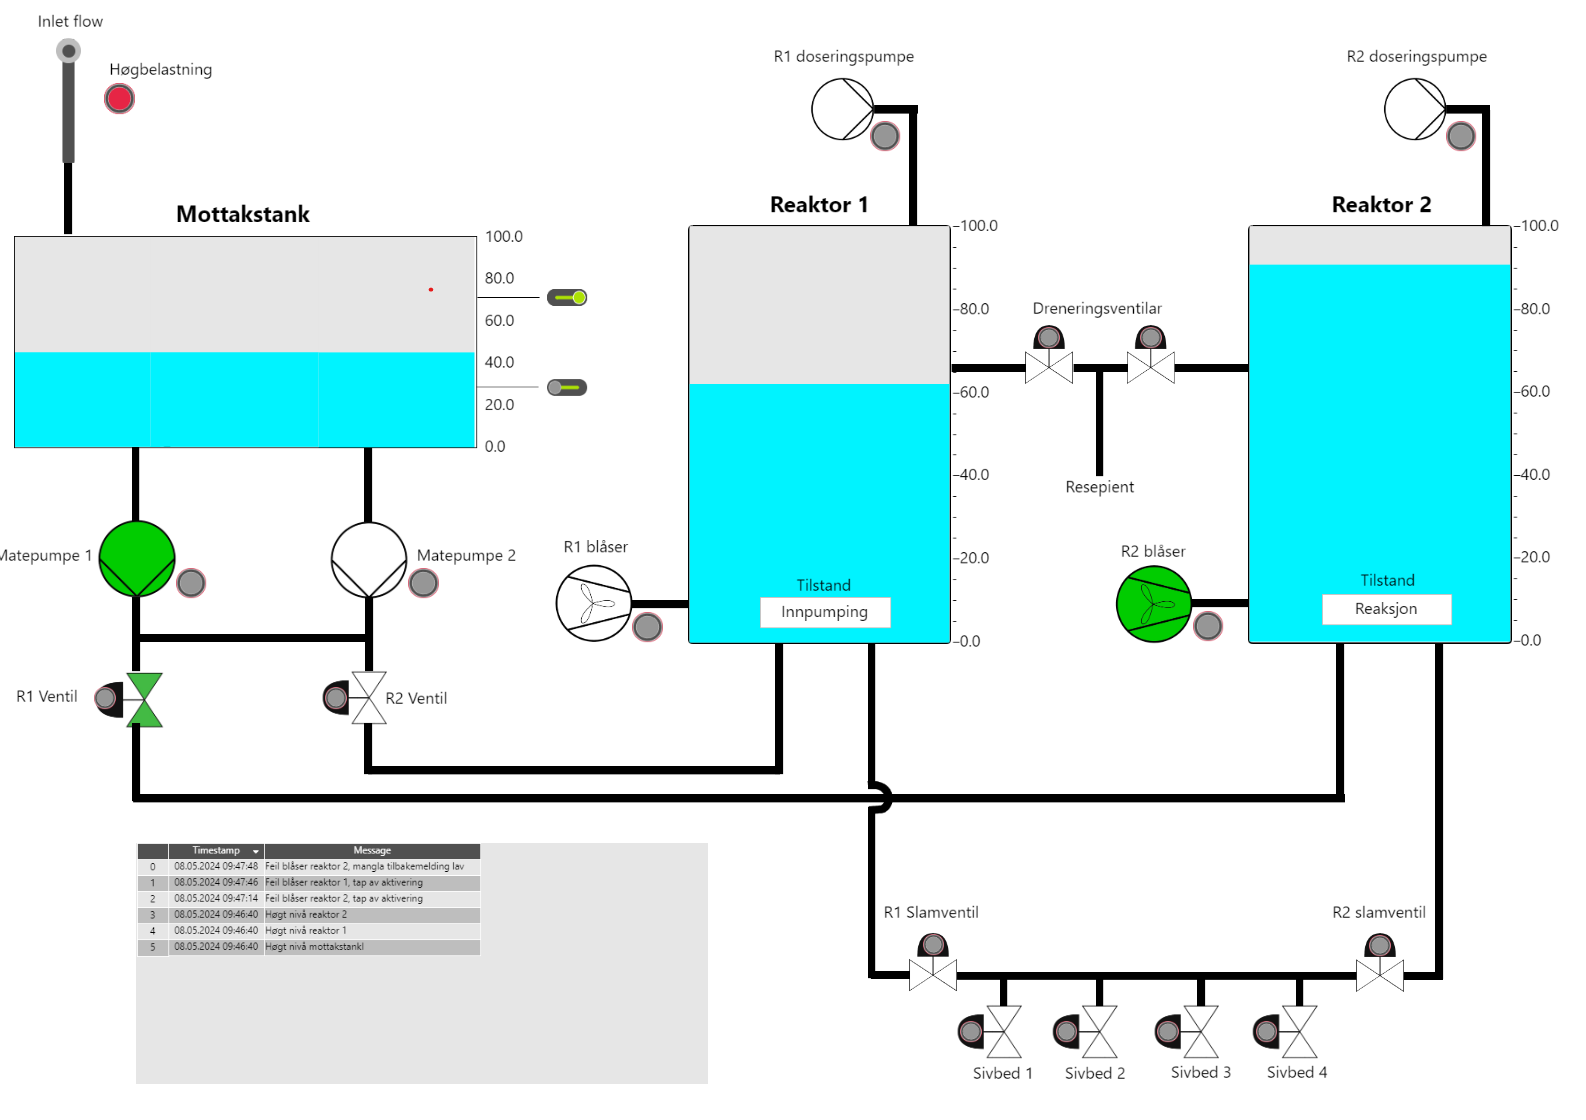
\includegraphics[scale=0.45]{Bilder/Simuleringsbilde.png}
    \caption{Oppsett av simuleringsvindauge}\label{fig:Simulering}
\end{figure}

\newpage

\subsection{Resultat}

Som forventa dukka det opp avvik i simuleringa.
Nokre av desse var av mindre betydning og blei utbetra undervegs, som t.d. skrivefeil, gløymde logiske operasjonar,
\gls{CFC}-koplingar som var feilplassert eller konfigurasjonsfeil. \newline
Andre avvik krevde meir arbeid og endring av program.
Den tiltenkte reaktorforriglinga som skulle hindre overgang til innpumpingssekvens, fungere ikkje.
Her var det naudsynt med ein ny løysning.

Simuleringa av programmet var vellykka og vi fekk samla verdifull informasjon. 
Den visuelle representasjonen var oversiktleg, der ein kunne sjå programmet i drift og enkelt oppdage feil. \newline
Vi konluderte at programmet i hovudsak fungerer som planlagt.
Programmet er no klar for ein meir omfattande simulering, der ein implementerer resterande funksjonar og fullfører fullskala test.

Simuleringsvideo er tilgjengeleg via Youtube. \newline
Link: \url{https://youtu.be/_2gtiXJDUyw}

%\includemedia[
  %width=0.5\linewidth,
  %height=0.45\linewidth,
  %activate=onclick,
  %flashvars={
    %modestbranding=1 % Fjern YouTube-logoen
    %&autohide=1 % Skjul kontrollene automatisk
    %&showinfo=0 % Skjul videotittel og annet informasjon
  %}
%]{}{https://youtu.be/_2gtiXJDUyw}





